% !TeX root = ../main.tex
\chapter{Unidad 1: Nociones básicas e introducción a la acústica}
\label{chap:unidad-1}

\section{Propósito y resultados de aprendizaje}
\label{sec:u1-proposito}

Esta unidad presenta el lenguaje físico y las herramientas matemáticas que se utilizarán a lo largo del libro. Su propósito no es desarrollar todavía toda la teoría de las ondas ni de los niveles acústicos, sino establecer una base común para describir fenómenos, interpretar ecuaciones y comunicar resultados con unidades correctas.

Al finalizar la unidad se espera que sea posible:

\begin{itemize}
    \item explicar el alcance general de la acústica mediante la relación entre fuente, medio y receptor;
    \item distinguir magnitudes fundamentales y derivadas del Sistema Internacional de Unidades (SI);
    \item diferenciar masa y peso, y relacionar distancia, tiempo, velocidad, aceleración, fuerza, presión y densidad;
    \item usar notación científica y comprobar la coherencia dimensional de una ecuación sencilla;
    \item interpretar una función y, cuando exista, su función inversa;
    \item utilizar seno, coseno y tangente en triángulos rectángulos y convertir entre grados y radianes;
    \item reconocer la relación inversa entre las funciones exponencial y logarítmica;
    \item explicar por qué el decibel expresa una relación logarítmica y no una magnitud física independiente;
    \item diferenciar una magnitud física de un atributo perceptual relacionado.
\end{itemize}

\section{Conocimientos previos}
\label{sec:u1-previos}

Se requiere operar con números enteros y decimales, fracciones, potencias y ecuaciones algebraicas de un paso. No se presupone conocimiento de cálculo diferencial. Cuando aparezca una razón de cambio, se interpretará primero como una comparación entre dos variaciones medibles.

\section{Una situación para comenzar}
\label{sec:u1-situacion}

Cuando una persona pronuncia una vocal, sus pliegues vocales y el tracto vocal participan en la producción de una señal. Esa señal se propaga por el aire, puede ser captada por un micrófono y finalmente puede producir una sensación sonora en quien escucha. En esta descripción aparecen tres componentes:

\begin{description}
    \item[\textbf{Fuente:}] sistema que origina la perturbación, como la voz, un parlante o un diapasón.
    \item[\textbf{Medio:}] material a través del cual se propaga la perturbación, como el aire, el agua o un sólido.
    \item[\textbf{Receptor:}] sistema que responde a la perturbación, como un micrófono, un instrumento de medición o el sistema auditivo.
\end{description}

Este esquema permite formular preguntas diferentes. La física puede estudiar qué magnitud cambia, con qué unidad se mide y cómo evoluciona. La percepción estudia qué experiencia produce esa señal en una persona. La práctica fonoaudiológica integra información física, perceptual y clínica, pero no las trata como si fueran equivalentes.

La figura~\ref{fig:fuente-medio-receptor} representa esta secuencia sin suponer que todo receptor sea una persona: un instrumento también puede responder a la perturbación.

\begin{figure}[htbp]
    \centering
    % Propósito: distinguir los tres componentes mínimos de una situación acústica.
% Origen: esquema conceptual fuente--medio--receptor de la Unidad 1.
% Descripción accesible: tres bloques, Fuente, Medio y Receptor, conectados en
% ese orden; la perturbación se origina en la fuente, se propaga por el medio y
% produce una respuesta en el receptor.
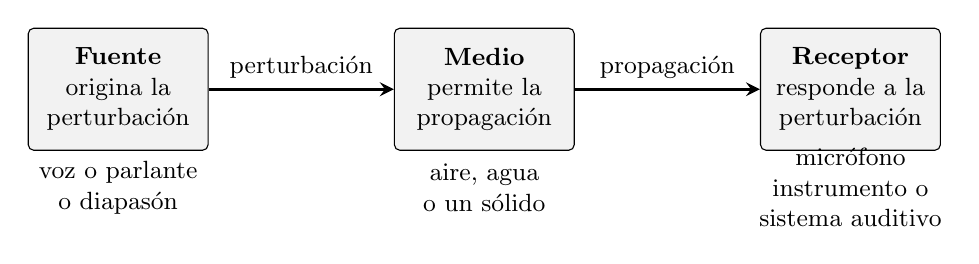
\begin{tikzpicture}[
    font=\small,
    >=stealth,
    bloque/.style={
        draw,
        rounded corners=2pt,
        text width=2.05cm,
        minimum height=1.55cm,
        align=center,
        fill=black!5
    }
]
    \node[bloque] (fuente) at (0,0)
        {\textbf{Fuente}\\origina la\\perturbación};
    \node[bloque] (medio) at (4.65,0)
        {\textbf{Medio}\\permite la\\propagación};
    \node[bloque] (receptor) at (9.3,0)
        {\textbf{Receptor}\\responde a la\\perturbación};

    \draw[->,very thick] (fuente.east) -- node[above]{perturbación} (medio.west);
    \draw[->,very thick] (medio.east) -- node[above]{propagación} (receptor.west);

    \node[align=center] at (0,-1.25) {voz o parlante\\o diapasón};
    \node[align=center] at (4.65,-1.25) {aire, agua\\o un sólido};
    \node[align=center] at (9.3,-1.25) {micrófono\\instrumento o\\sistema auditivo};
\end{tikzpicture}

    \caption{Modelo mínimo fuente--medio--receptor. La fuente origina una perturbación, el medio permite su propagación y el receptor produce una respuesta. Los ejemplos indican posibles sistemas en cada función y no constituyen una lista exhaustiva. Elaboración propia.}
    \label{fig:fuente-medio-receptor}
\end{figure}

\section{Alcance de la acústica y relación con Fonoaudiología}
\label{sec:u1-alcance}

La \textbf{acústica} estudia la producción, la propagación, la recepción, el control y los efectos del sonido y de otras vibraciones mecánicas. Incluye tanto la descripción física de las señales como el estudio de los sistemas que las producen, transmiten o reciben.

En Fonoaudiología, este enfoque aporta herramientas para:

\begin{itemize}
    \item describir estímulos y respuestas utilizados en evaluaciones auditivas;
    \item analizar señales de voz en el tiempo y en frecuencia;
    \item comprender, a nivel funcional, la entrada y la salida de dispositivos electroacústicos;
    \item identificar condiciones físicas de un ambiente que pueden afectar una medición.
\end{itemize}

Estas aplicaciones no reemplazan el razonamiento clínico. Una medición acústica describe una señal o la respuesta de un sistema; su interpretación diagnóstica exige información adicional y se abordará en unidades posteriores.

\section{El sonido como perturbación mecánica}
\label{sec:u1-onda-mecanica}

El sonido requiere un medio material para propagarse. En el aire, una fuente sonora produce pequeñas variaciones locales de presión y movimiento de las partículas. Cada región del medio interactúa con las regiones vecinas, de modo que la perturbación avanza aunque las partículas no viajen junto con ella desde la fuente hasta el receptor.

Conviene separar dos ideas:

\begin{itemize}
    \item la \textbf{oscilación local} describe el movimiento de una parte del medio alrededor de una posición de equilibrio;
    \item la \textbf{propagación} describe el avance de la perturbación y de la energía asociada a través del medio.
\end{itemize}

En gases y líquidos, las ondas sonoras se propagan mediante compresiones y rarefacciones, por lo que se describen como longitudinales. Los sólidos pueden admitir ondas longitudinales y transversales porque resisten tanto deformaciones de compresión como de corte. La relación entre estas ondas y los mecanismos de conducción ósea no se reduce a un único tipo de movimiento y se estudiará más adelante.

La descripción matemática de la oscilación, la propagación y los parámetros de una onda se desarrolla en la Unidad~\ref{chap:unidad-3}. En esta unidad basta con conservar la idea central: una onda mecánica es una perturbación que se propaga en un medio, no un transporte neto de materia desde la fuente hasta el receptor.

\subsection{Actividad de observación}
\label{sec:u1-actividad-onda}

Puede colocarse un resorte largo sobre una mesa y marcar una de sus espiras con una cinta liviana. Después de estirarlo moderadamente, se produce un pulso pequeño empujando un extremo en la dirección del resorte.

\begin{enumerate}
    \item Se observa que la zona comprimida avanza a lo largo del resorte.
    \item Se observa por separado el movimiento de la espira marcada.
    \item Se compara la distancia recorrida por la perturbación con el desplazamiento de la espira.
\end{enumerate}

La observación esperada es que la perturbación recorra una distancia mucho mayor que la espira marcada. El resorte es un modelo visible de propagación; no reproduce todas las propiedades del sonido en el aire. Debe evitarse estirarlo en exceso o soltarlo en dirección a otra persona.

\section{Magnitudes físicas y Sistema Internacional}
\label{sec:u1-si}

\subsection{Magnitud, valor y unidad}
\label{sec:u1-magnitud-unidad}

Una \textbf{magnitud física} es una propiedad que puede medirse o calcularse. El resultado se expresa mediante un valor numérico y una unidad. Por ejemplo, en \(d=2\,\text{m}\), el símbolo \(d\) representa una distancia, \(2\) es el valor numérico y el metro (\(\text{m}\)) es la unidad.

El SI comprende siete unidades básicas definidas a partir de siete constantes definitorias; las unidades derivadas se expresan como productos de potencias de las unidades básicas~\cite{bipmSI2026}. La tabla~\ref{tab:u1-magnitudes-fundamentales} presenta las siete magnitudes fundamentales y sus unidades.

\begin{table}[htbp]
    \centering
    \begin{tabular}{|l|c|c|}
        \hline
        \textbf{Magnitud fundamental} & \textbf{Símbolo usual} & \textbf{Unidad SI} \\
        \hline
        Tiempo & \(t\) & segundo (\(\text{s}\)) \\
        Longitud & \(l\) & metro (\(\text{m}\)) \\
        Masa & \(m\) & kilogramo (\(\text{kg}\)) \\
        Corriente eléctrica & \(I\) & ampere (\(\text{A}\)) \\
        Temperatura termodinámica & \(T\) & kelvin (\(\text{K}\)) \\
        Cantidad de sustancia & \(n\) & mol (\(\text{mol}\)) \\
        Intensidad luminosa & \(I_\mathrm{v}\) & candela (\(\text{cd}\)) \\
        \hline
    \end{tabular}
    \caption{Magnitudes fundamentales y unidades del Sistema Internacional.}
    \label{tab:u1-magnitudes-fundamentales}
\end{table}

Para temperaturas ambientales se emplearán por defecto grados Celsius (\(^{\circ}\text{C}\)). El kelvin se reservará para temperaturas absolutas y ecuaciones termodinámicas. Por ejemplo, se escribe \(20\,^{\circ}\text{C}\), con un espacio entre el valor y la unidad; no se escribe ``20 grados kelvin'' ni \(20\,^{\circ}\text{K}\).

\subsection{Magnitudes derivadas}
\label{sec:u1-magnitudes-derivadas}

Una magnitud derivada se define mediante otras magnitudes. La tabla~\ref{tab:u1-magnitudes-derivadas} resume algunas que se utilizarán en el libro.

En estas expresiones:

\begin{itemize}
    \item \(d\) es la distancia recorrida, medida en metros (\(\text{m}\));
    \item \(\Delta t\) es el intervalo de tiempo, medido en segundos (\(\text{s}\));
    \item \(\Delta v\) es el cambio de velocidad, medido en metros por segundo (\(\text{m}/\text{s}\));
    \item \(m\) es la masa, medida en kilogramos (\(\text{kg}\));
    \item \(a\) es la aceleración, medida en metros por segundo cuadrado (\(\text{m}/\text{s}^{2}\));
    \item \(F_\perp\) es la componente de la fuerza perpendicular a una superficie, medida en newtons (\(\text{N}\));
    \item \(A\) es el área de la superficie, medida en metros cuadrados (\(\text{m}^{2}\));
    \item \(V\) es el volumen, medido en metros cúbicos (\(\text{m}^{3}\));
    \item \(N\) es el número de ciclos observados y no tiene unidad.
\end{itemize}

\begin{table}[htbp]
    \centering
    \setlength{\tabcolsep}{4pt}
    \begin{tabular}{|>{\raggedright\arraybackslash}p{0.22\textwidth}|c|>{\raggedright\arraybackslash}p{0.25\textwidth}|>{\raggedright\arraybackslash}p{0.25\textwidth}|}
        \hline
        \textbf{Magnitud} & \textbf{Símbolo} & \textbf{Relación básica} & \textbf{Unidad SI} \\
        \hline
        Rapidez media & \(v_\mathrm{med}\) & \(v_\mathrm{med}=d/\Delta t\) & metro por segundo (\(\text{m}/\text{s}\)) \\
        Aceleración media & \(a_\mathrm{med}\) & \(a_\mathrm{med}=\Delta v/\Delta t\) & metro por segundo cuadrado (\(\text{m}/\text{s}^{2}\)) \\
        Fuerza & \(F\) & \(F=ma\), en el modelo indicado & newton (\(\text{N}\)) \\
        Presión media & \(p\) & \(p=F_\perp/A\) & pascal (\(\text{Pa}\)) \\
        Densidad de masa & \(\rho\) & \(\rho=m/V\) & kilogramo por metro cúbico (\(\text{kg}/\text{m}^{3}\)) \\
        Frecuencia & \(f\) & \(f=N/\Delta t\) & hertz (\(\text{Hz}\)) \\
        \hline
    \end{tabular}
    \caption{Algunas magnitudes derivadas, relaciones de definición y unidades SI.}
    \label{tab:u1-magnitudes-derivadas}
\end{table}

La expresión \(F=ma\) se utilizará como forma introductoria de la segunda ley de Newton para un cuerpo de masa constante y una fuerza neta. Sus condiciones y aplicaciones se desarrollan en la Unidad~\ref{chap:unidad-2}.

\subsection{Masa y peso}
\label{sec:u1-masa-peso}

La \textbf{masa} caracteriza la inercia de un cuerpo y se mide en kilogramos (\(\text{kg}\)). El \textbf{peso} es la fuerza gravitatoria que actúa sobre ese cuerpo y se mide en newtons (\(\text{N}\)). No son la misma magnitud, aunque en el lenguaje cotidiano se utilice la palabra ``peso'' para informar una masa.

Si \(F_\mathrm{g}\) representa el peso, \(m\) la masa y \(g\) la aceleración gravitatoria local, entonces:

\begin{equation}
    F_\mathrm{g}=mg.
    \label{eq:u1-peso}
\end{equation}

La masa de un cuerpo puede conservarse aunque cambie el valor de \(g\); en ese caso cambia su peso. Esta distinción será necesaria para interpretar correctamente fuerzas y aceleraciones.

\subsection{Rapidez, velocidad y velocidad de propagación}
\label{sec:u1-velocidades}

La rapidez informa cuánta distancia se recorre por unidad de tiempo y no incluye dirección. La velocidad es una magnitud vectorial: incluye módulo, dirección y sentido. En problemas unidimensionales ambas pueden tener el mismo valor numérico, pero representan conceptos distintos.

En acústica también aparece la \textbf{velocidad de propagación}, que describe cuánto avanza una perturbación por unidad de tiempo. Se utilizará el símbolo \(c\), medido en metros por segundo (\(\text{m}/\text{s}\)), para diferenciarla del movimiento local de las partículas del medio.

Como valor de referencia didáctico, para aire cercano a \(20\,^{\circ}\text{C}\) suele emplearse \(c\approx343\,\text{m}/\text{s}\)~\cite{cramer1993}. Este valor no es universal: depende de las propiedades y del estado del medio.

\subsection{Ejemplo resuelto: tiempo de propagación}
\label{sec:u1-ejemplo-tiempo}

Supongamos que una perturbación recorre una distancia \(d=100\,\text{m}\) en aire y adoptamos \(c=343\,\text{m}/\text{s}\). Primero se interpreta la relación física: si se conocen la distancia y la rapidez de propagación, el tiempo se obtiene dividiendo distancia por rapidez.

Si \(t\) es el tiempo de propagación, medido en segundos (\(\text{s}\)), entonces:

\[
    t=\frac{d}{c}
     =\frac{100\,\text{m}}{343\,\text{m}/\text{s}}
     \approx0{,}29\,\text{s}
     =290\,\text{ms}.
\]

Las unidades confirman el resultado:

\[
    \frac{\text{m}}{\text{m}/\text{s}}=\text{s}.
\]

El cálculo representa un modelo de propagación con velocidad constante. No describe por sí solo reflexiones, variaciones atmosféricas ni la respuesta de un receptor.

\section{Notación científica, prefijos y análisis dimensional}
\label{sec:u1-notacion-dimensional}

\subsection{Notación científica}
\label{sec:u1-notacion-cientifica}

La notación científica expresa un número como el producto entre un coeficiente y una potencia de diez:

\[
    a\times10^{n},
\]

donde \(a\) es un número cuyo valor absoluto es mayor o igual que \(1\) y menor que \(10\), y \(n\) es un número entero. Por ejemplo:

\[
    0{,}000020\,\text{Pa}
    =2{,}0\times10^{-5}\,\text{Pa}
    =20\,\mu\text{Pa}.
\]

El prefijo micro, de símbolo \(\mu\), representa \(10^{-6}\); mili (\(\text{m}\)) representa \(10^{-3}\) y kilo (\(\text{k}\)) representa \(10^{3}\). El contexto permite distinguir el símbolo de una unidad del símbolo de una magnitud: por ejemplo, \(\text{m}\) puede ser el metro como unidad, mientras que \(m\) en cursiva puede representar la masa.

\subsection{Análisis dimensional}
\label{sec:u1-analisis-dimensional}

Una ecuación física solo puede ser correcta si ambos miembros tienen dimensiones compatibles. Este control no demuestra que la ecuación sea verdadera, pero permite detectar muchos errores.

Por ejemplo, la presión media se define como \(p=F_\perp/A\). La fuerza se mide en newtons, y:

\[
    1\,\text{N}=1\,\text{kg}\,\text{m}/\text{s}^{2}.
\]

Por lo tanto:

\[
    \frac{\text{N}}{\text{m}^{2}}
    =\frac{\text{kg}\,\text{m}/\text{s}^{2}}{\text{m}^{2}}
    =\frac{\text{kg}}{\text{m}\,\text{s}^{2}}
    =\text{Pa}.
\]

Si una suma combina directamente metros con segundos, o si una ecuación de tiempo produce unidades de metros, existe una inconsistencia que debe corregirse.

La figura~\ref{fig:magnitudes-fundamentales-derivadas} reúne las mismas relaciones desde el punto de vista dimensional. Cada división por un intervalo de tiempo incorpora un factor \(T^{-1}\); dividir por un área o un volumen incorpora, respectivamente, \(L^{-2}\) o \(L^{-3}\).

\begin{figure}[htbp]
    \centering
    % Propósito: mostrar cómo magnitudes derivadas se construyen combinando
% dimensiones de masa [M], longitud [L] y tiempo [T].
% Origen: v=d/Delta t, a=Delta v/Delta t, F=ma, p=F/A,
% rho=m/V y f=N/Delta t, con N adimensional.
% Descripción accesible: cuatro cadenas muestran que longitud dividida por
% tiempo produce rapidez y, al dividir otra vez por tiempo, aceleración; masa
% por aceleración produce fuerza y fuerza dividida por área produce presión;
% masa dividida por volumen produce densidad; uno dividido por tiempo produce
% frecuencia.
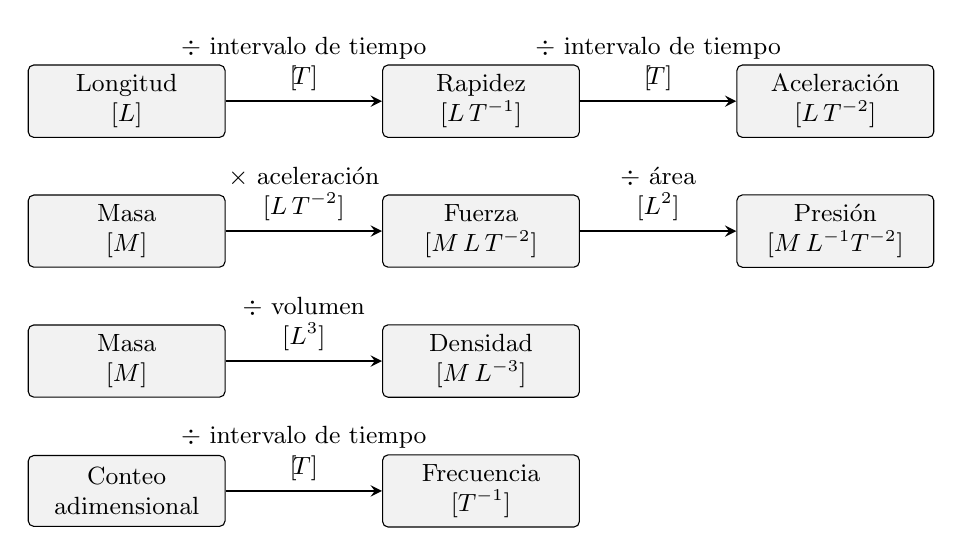
\begin{tikzpicture}[
    font=\small,
    >=stealth,
    magnitud/.style={
        draw,
        rounded corners=2pt,
        minimum width=2.5cm,
        minimum height=0.9cm,
        align=center,
        fill=black!5
    }
]
    \node[magnitud] (longitud) at (0,0) {Longitud\\\([L]\)};
    \node[magnitud] (rapidez) at (4.5,0) {Rapidez\\\([L\,T^{-1}]\)};
    \node[magnitud] (aceleracion) at (9,0) {Aceleración\\\([L\,T^{-2}]\)};
    \draw[->,thick] (longitud.east) -- node[above,align=center]
        {\(\div\) intervalo de tiempo\\\([\!T]\)} (rapidez.west);
    \draw[->,thick] (rapidez.east) -- node[above,align=center]
        {\(\div\) intervalo de tiempo\\\([\!T]\)} (aceleracion.west);

    \node[magnitud] (masa-f) at (0,-1.65) {Masa\\\([M]\)};
    \node[magnitud] (fuerza) at (4.5,-1.65) {Fuerza\\\([M\,L\,T^{-2}]\)};
    \node[magnitud] (presion) at (9,-1.65) {Presión\\\([M\,L^{-1}T^{-2}]\)};
    \draw[->,thick] (masa-f.east) -- node[above,align=center]
        {\(\times\) aceleración\\\([L\,T^{-2}]\)} (fuerza.west);
    \draw[->,thick] (fuerza.east) -- node[above,align=center]
        {\(\div\) área\\\([L^{2}]\)} (presion.west);

    \node[magnitud] (masa-rho) at (0,-3.3) {Masa\\\([M]\)};
    \node[magnitud] (densidad) at (4.5,-3.3) {Densidad\\\([M\,L^{-3}]\)};
    \draw[->,thick] (masa-rho.east) -- node[above,align=center]
        {\(\div\) volumen\\\([L^{3}]\)} (densidad.west);

    \node[magnitud] (uno) at (0,-4.95) {Conteo\\adimensional};
    \node[magnitud] (frecuencia) at (4.5,-4.95) {Frecuencia\\\([T^{-1}]\)};
    \draw[->,thick] (uno.east) -- node[above,align=center]
        {\(\div\) intervalo de tiempo\\\([\!T]\)} (frecuencia.west);
\end{tikzpicture}

    \caption{Construcción dimensional de algunas magnitudes derivadas a partir de masa \([M]\), longitud \([L]\) y tiempo \([T]\). Las cadenas muestran operaciones entre dimensiones, no valores medidos. Elaboración propia a partir de las definiciones de esta unidad.}
    \label{fig:magnitudes-fundamentales-derivadas}
\end{figure}

\section{Herramientas matemáticas básicas}
\label{sec:u1-herramientas}

\subsection{Variables, relaciones y funciones}
\label{sec:u1-funciones}

Una variable representa una cantidad que puede tomar distintos valores. Una \textbf{función} asigna a cada valor permitido de una variable de entrada un único valor de salida. Se escribe:

\[
    y=f(x),
\]

donde \(x\) es la variable independiente, \(y\) es la variable dependiente y \(f\) indica la regla de asignación. El conjunto de valores permitidos para \(x\) se denomina dominio.

Si una perturbación se propaga con rapidez constante \(c\), la distancia \(d\), medida en metros (\(\text{m}\)), puede expresarse como función del tiempo \(t\), medido en segundos (\(\text{s}\)):

\[
    d(t)=ct.
\]

Esta ecuación no afirma que toda propagación tenga velocidad constante. Describe un modelo válido cuando esa aproximación es adecuada.

\subsection{Función inversa}
\label{sec:u1-funcion-inversa}

Una función inversa permite recuperar la entrada a partir de la salida. No toda función posee inversa en todo su dominio: para que exista, cada salida considerada debe corresponder a una única entrada.

Para el modelo \(d(t)=ct\), con \(c>0\) constante y \(t\geq0\), la función inversa permite calcular el tiempo a partir de la distancia:

\[
    t(d)=\frac{d}{c}.
\]

No debe confundirse la función inversa \(f^{-1}\) con el recíproco \(1/f\). Por ejemplo, si \(f(x)=2x\), entonces \(f^{-1}(x)=x/2\), mientras que \(1/f(x)=1/(2x)\).

La figura~\ref{fig:funcion-directa-inversa} aplica la ida y la vuelta al modelo \(d(t)=ct\): la función directa calcula una distancia y la inversa recupera el tiempo correspondiente.

\begin{figure}[htbp]
    \centering
    % Propósito: mostrar que una función inversa recupera la variable de entrada.
% Origen: d(t)=ct y t(d)=d/c para c=4 m/s, t=3 s y d=12 m.
% Descripción accesible: un bloque de tiempo de 3 s se conecta con uno de
% distancia de 12 m mediante una flecha directa d=ct; una segunda flecha en
% sentido contrario, t=d/c, recupera el tiempo. En ambos casos c=4 m/s.
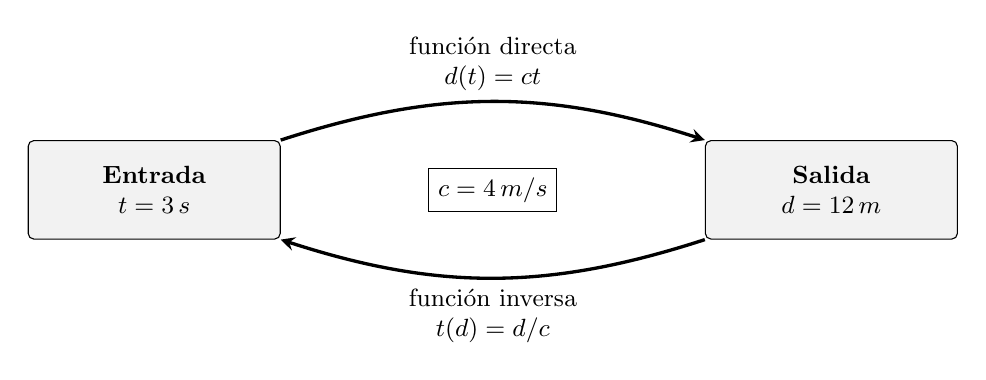
\begin{tikzpicture}[
    font=\small,
    >=stealth,
    valor/.style={
        draw,
        rounded corners=2pt,
        minimum width=3.2cm,
        minimum height=1.25cm,
        align=center,
        fill=black!5
    }
]
    \node[valor] (tiempo) at (0,0) {\textbf{Entrada}\\\(t=3\,\text{s}\)};
    \node[valor] (distancia) at (8.6,0) {\textbf{Salida}\\\(d=12\,\text{m}\)};

    \draw[->,very thick] (tiempo.north east) to[bend left=18]
        node[above,align=center]{función directa\\\(d(t)=ct\)}
        (distancia.north west);
    \draw[->,very thick] (distancia.south west) to[bend left=18]
        node[below,align=center]{función inversa\\\(t(d)=d/c\)}
        (tiempo.south east);

    \node[draw,align=center,fill=white] at (4.3,0)
        {\(c=4\,\text{m}/\text{s}\)};
\end{tikzpicture}

    \caption{Función directa e inversa para un movimiento uniforme con \(c=4\,\text{m}/\text{s}\). A partir de \(t=3\,\text{s}\), la función directa obtiene \(d=12\,\text{m}\); la función inversa recupera el valor inicial del tiempo. Elaboración propia.}
    \label{fig:funcion-directa-inversa}
\end{figure}

\subsection{Trigonometría}
\label{sec:u1-trigonometria}

La trigonometría relaciona ángulos y longitudes. En un triángulo rectángulo se consideran un ángulo \(\theta\), el cateto opuesto a ese ángulo, el cateto adyacente y la hipotenusa. Las razones trigonométricas básicas son:

\[
    \sin\theta
    =\frac{\text{cateto opuesto}}{\text{hipotenusa}},
    \qquad
    \cos\theta
    =\frac{\text{cateto adyacente}}{\text{hipotenusa}},
\]

\[
    \tan\theta
    =\frac{\text{cateto opuesto}}{\text{cateto adyacente}}
    =\frac{\sin\theta}{\cos\theta},
\]

siempre que \(\cos\theta\neq0\) para la tangente.

Los ángulos pueden expresarse en grados (\(^{\circ}\)) o en radianes (\(\text{rad}\)). Una vuelta completa equivale a:

\[
    360^{\circ}=2\pi\,\text{rad}.
\]

Por lo tanto:

\[
    90^{\circ}=\frac{\pi}{2}\,\text{rad}.
\]

Los ángulos \(640^{\circ}\) y \(280^{\circ}\) tienen la misma orientación final porque difieren en una vuelta completa:

\[
    640^{\circ}\equiv280^{\circ}\pmod{360^{\circ}},
    \qquad
    280^{\circ}=\frac{14\pi}{9}\,\text{rad}.
\]

El círculo trigonométrico permite extender seno y coseno más allá de los triángulos rectángulos y será útil para describir fenómenos periódicos. La ecuación completa de una oscilación sinusoidal, su amplitud, frecuencia y fase pertenecen a la Unidad~\ref{chap:unidad-3}.

La figura~\ref{fig:circulo-trigonometrico} muestra que, en un círculo de radio unitario, el coseno y el seno pueden leerse como las proyecciones horizontal y vertical del punto determinado por el ángulo.

\begin{figure}[htbp]
    \centering
    % Propósito: relacionar un ángulo del círculo unitario con coseno y seno.
% Origen: x=cos(theta), y=sin(theta) para un radio unitario.
% Descripción accesible: en un círculo de radio uno, un radio forma un ángulo
% theta con el eje horizontal. La proyección horizontal del punto extremo mide
% cos(theta) y la proyección vertical mide sin(theta).
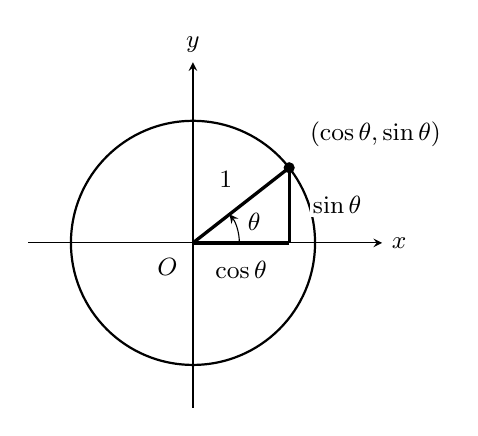
\begin{tikzpicture}[font=\small,>=stealth,scale=1.55]
    \draw[->] (-1.35,0) -- (1.55,0) node[right]{\(x\)};
    \draw[->] (0,-1.35) -- (0,1.48) node[above]{\(y\)};
    \draw[thick] (0,0) circle (1);

    \coordinate (P) at (38:1);
    \coordinate (Px) at ({cos(38)},0);

    \draw[very thick] (0,0) -- node[pos=0.55,above left=1pt]{\(1\)} (P);
    \draw[dashed] (P) -- (Px);
    \draw[very thick] (0,0) --
        node[midway,below=5pt,fill=white,inner sep=1pt]{\(\cos\theta\)} (Px);
    \draw[very thick] (Px) --
        node[midway,right=7pt,fill=white,inner sep=1pt]{\(\sin\theta\)} (P);
    \fill (P) circle (1.3pt);

    \draw[->] (0.38,0) arc[start angle=0,end angle=38,radius=0.38];
    \node at (19:0.53) {\(\theta\)};

    \node[below left=2pt] at (0,0) {\(O\)};
    \node[above right=4pt] at (P) {\((\cos\theta,\sin\theta)\)};
\end{tikzpicture}

    \caption{Círculo trigonométrico de radio \(1\). Para un ángulo \(\theta\), el punto del círculo tiene coordenadas adimensionales \((\cos\theta,\sin\theta)\). Elaboración propia.}
    \label{fig:circulo-trigonometrico}
\end{figure}

\subsection{Función exponencial}
\label{sec:u1-exponencial}

Una función exponencial tiene la forma:

\[
    y=a^{x},
\]

donde la base \(a\) es positiva y distinta de \(1\), y \(x\) es el exponente. Si \(a>1\), la función crece al aumentar \(x\); si \(0<a<1\), decrece.

Por ejemplo:

\[
    10^{3}=1000,
    \qquad
    10^{-3}=0{,}001.
\]

Las funciones exponenciales resultan útiles para representar procesos en los que un cambio multiplicativo se repite.

\subsection{Logaritmos}
\label{sec:u1-logaritmos}

El logaritmo responde a la pregunta: ¿a qué exponente debe elevarse una base para obtener un número? Para una base \(a>0\), \(a\neq1\), y un argumento \(x>0\):

\[
    y=\log_{a}(x)
    \quad\Longleftrightarrow\quad
    a^{y}=x.
\]

Por ejemplo:

\[
    \log_{10}(1000)=3
    \quad\Longleftrightarrow\quad
    10^{3}=1000.
\]

La función logarítmica es la inversa de la función exponencial con la misma base. Además, el argumento de un logaritmo aplicado a magnitudes físicas debe ser adimensional; por eso se utilizan razones entre magnitudes de la misma clase y con las mismas unidades.

\subsection{Anticipo: relaciones expresadas en decibeles}
\label{sec:u1-decibel}

El decibel, de símbolo \(\text{dB}\), se utiliza para expresar el valor de una relación logarítmica especificada~\cite{nistSP811}. No es una unidad absoluta de presión, intensidad o potencia. Para interpretar un valor en decibeles se debe conocer qué magnitud se compara y cuál es la referencia.

Para una magnitud de tipo potencia \(Q\) y una referencia \(Q_0\) de la misma clase y expresada en la misma unidad, puede definirse:

\begin{equation}
    L_Q=10\log_{10}\left(\frac{Q}{Q_0}\right).
    \label{eq:u1-relacion-db}
\end{equation}

En la ecuación~\eqref{eq:u1-relacion-db}, \(L_Q\) es el nivel de la magnitud \(Q\) respecto de \(Q_0\), expresado en decibeles. La razón \(Q/Q_0\) no tiene unidad.

Si \(Q/Q_0=100\), entonces:

\[
    L_Q=10\log_{10}(100)
       =10\times2
       =20\,\text{dB}.
\]

La figura~\ref{fig:escala-lineal-logaritmica} compara la ubicación de las razones \(1\), \(10\), \(100\) y \(1000\) en ambas representaciones. En la escala logarítmica, multiplicar la razón por \(10\) produce siempre el mismo incremento de \(10\,\text{dB}\).

\begin{figure}[htbp]
    \centering
    % Propósito: comparar la separación espacial de razones en una escala lineal
% con la separación uniforme de sus logaritmos.
% Origen: L_Q=10 log10(Q/Q0), para Q/Q0=1,10,100,1000.
% Descripción accesible: en una escala lineal de cero a mil, las razones 1 y 10
% quedan casi superpuestas cerca del origen y 100 permanece en la primera
% décima parte. En la representación logarítmica, 1, 10, 100 y 1000 quedan
% igualmente espaciados y corresponden a 0, 10, 20 y 30 dB.
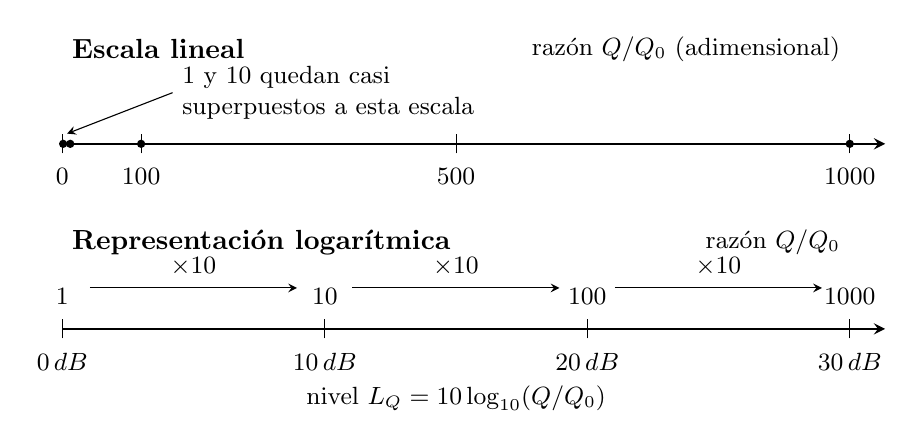
\begin{tikzpicture}[font=\small,>=stealth,x=1cm,y=1cm]
    % Escala lineal: encabezado, anotación y eje ocupan bandas distintas.
    \node[anchor=west,font=\bfseries] at (0,3.25) {Escala lineal};
    \node[anchor=east] at (10,3.25)
        {razón \(Q/Q_0\) (adimensional)};
    \draw[->,thick] (0,2.05) -- (10.45,2.05);
    \foreach \x/\etiqueta in {0/0,1/100,5/500,10/1000}{
        \draw (\x,1.93) -- (\x,2.17);
        \node[below=2pt] at (\x,1.93) {\etiqueta};
    }
    \fill (0.01,2.05) circle (1.5pt);
    \fill (0.1,2.05) circle (1.5pt);
    \fill (1,2.05) circle (1.5pt);
    \fill (10,2.05) circle (1.5pt);
    \node[anchor=west,align=left] (anotacion) at (1.40,2.70)
        {\(1\) y \(10\) quedan casi\\superpuestos a esta escala};
    \draw[->] (anotacion.west) -- (0.06,2.18);

    % Representación logarítmica: las razones, los niveles y los factores
    % multiplicativos se colocan en franjas verticales independientes.
    \node[anchor=west,font=\bfseries] at (0,0.80)
        {Representación logarítmica};
    \node[anchor=east] at (10,0.80) {razón \(Q/Q_0\)};
    \draw[->,thick] (0,-0.30) -- (10.45,-0.30);
    \foreach \x/\razon/\nivel in {
        0/1/0,
        3.333/10/10,
        6.666/100/20,
        10/1000/30
    }{
        \draw (\x,-0.42) -- (\x,-0.18);
        \node[above=2pt] at (\x,-0.18) {\(\razon\)};
        \node[below=2pt] at (\x,-0.42) {\(\nivel\,\text{dB}\)};
    }
    \node at (5,-1.18) {nivel \(L_Q=10\log_{10}(Q/Q_0)\)};

    \foreach \x in {0,3.333,6.666}{
        \draw[->] (\x+0.35,0.22) -- (\x+2.98,0.22)
            node[midway,above=1pt]{\(\times10\)};
    }
\end{tikzpicture}

    \caption{Comparación de una escala lineal con la representación logarítmica definida por \(L_Q=10\log_{10}(Q/Q_0)\). Las razones sucesivas por un factor \(10\) quedan igualmente separadas en la representación logarítmica y corresponden a incrementos de \(10\,\text{dB}\). Elaboración propia.}
    \label{fig:escala-lineal-logaritmica}
\end{figure}

La definición del nivel de presión sonora, el uso del factor \(20\), los valores eficaces y las referencias acústicas se desarrollan en la Unidad~\ref{chap:unidad-4}. También se distinguirán allí los niveles de presión, intensidad y potencia.

\section{Magnitudes físicas y atributos perceptuales}
\label{sec:u1-fisico-perceptual}

Una magnitud física se define mediante un procedimiento de medición y una unidad. Un atributo perceptual describe una experiencia y depende de la señal, del oyente y del contexto.

\begin{table}[htbp]
    \centering
    \setlength{\tabcolsep}{4pt}
    \begin{tabular}{|>{\raggedright\arraybackslash}p{0.26\textwidth}|>{\raggedright\arraybackslash}p{0.29\textwidth}|>{\raggedright\arraybackslash}p{0.31\textwidth}|}
        \hline
        \textbf{Descripción física} & \textbf{Correlato perceptual} & \textbf{Aclaración} \\
        \hline
        Frecuencia (\(\text{Hz}\)) & Altura tonal o \emph{pitch} & No son sinónimos; la percepción depende de la señal y del oyente. \\
        Amplitud (con magnitud y unidad explícitas) & Sonoridad & La amplitud debe indicar qué magnitud representa y con qué unidad. \\
        Espectro y evolución temporal & Timbre & El timbre no se reduce a una única componente espectral. \\
        Control de ganancia de un equipo & ``Volumen'' en uso cotidiano & El control modifica el sistema; ``volumen'' no es una magnitud acústica. \\
        \hline
    \end{tabular}
    \caption{Separación entre descripciones físicas, atributos perceptuales y controles técnicos.}
    \label{tab:u1-fisico-perceptual}
\end{table}

Para tonos simples dentro de condiciones comparables, un aumento de frecuencia suele asociarse con un aumento de la altura tonal percibida, pero frecuencia y \emph{pitch} no son equivalentes~\cite{oxenham2018}. De manera análoga, aumentar una amplitud o un nivel físico puede modificar la sonoridad, pero no permite predecirla por sí solo.

\section{Ejemplos resueltos}
\label{sec:u1-ejemplos}

\subsection{Masa y peso}
\label{sec:u1-ejemplo-peso}

Una masa \(m=2{,}5\,\text{kg}\) se encuentra en una región donde se adopta \(g=9{,}8\,\text{m}/\text{s}^{2}\) como dato del problema. El peso \(F_\mathrm{g}\), medido en newtons (\(\text{N}\)), se obtiene con la ecuación~\eqref{eq:u1-peso}:

\[
    F_\mathrm{g}
    =(2{,}5\,\text{kg})(9{,}8\,\text{m}/\text{s}^{2})
    =24{,}5\,\text{N}.
\]

El resultado no cambia la masa: \(m\) continúa siendo \(2{,}5\,\text{kg}\). Lo que se calculó es una fuerza.

\subsection{Fuerza, área y presión}
\label{sec:u1-ejemplo-presion}

Una fuerza perpendicular \(F_\perp=0{,}60\,\text{N}\) se distribuye uniformemente sobre un área \(A=0{,}030\,\text{m}^{2}\). La presión media \(p\), medida en pascales (\(\text{Pa}\)), es:

\[
    p=\frac{F_\perp}{A}
     =\frac{0{,}60\,\text{N}}{0{,}030\,\text{m}^{2}}
     =20\,\text{Pa}.
\]

Este ejemplo ilustra la definición mecánica de presión. No permite calcular una intensidad acústica sin información adicional sobre el campo y el medio.

\subsection{Función directa e inversa}
\label{sec:u1-ejemplo-inversa}

En un modelo de movimiento uniforme se adopta \(c=4\,\text{m}/\text{s}\). La distancia recorrida en función del tiempo es:

\[
    d(t)=ct=(4\,\text{m}/\text{s})t.
\]

Para \(t=3\,\text{s}\):

\[
    d(3\,\text{s})=(4\,\text{m}/\text{s})(3\,\text{s})=12\,\text{m}.
\]

La función inversa permite preguntar cuánto tiempo se necesita para recorrer una distancia \(d=20\,\text{m}\):

\[
    t(d)=\frac{d}{c},
    \qquad
    t(20\,\text{m})
    =\frac{20\,\text{m}}{4\,\text{m}/\text{s}}
    =5\,\text{s}.
\]

\section{Relación con la práctica fonoaudiológica}
\label{sec:u1-relacion-fono}

Las herramientas de esta unidad reaparecen en distintos contextos:

\begin{itemize}
    \item en una audiometría se deben distinguir la frecuencia del estímulo, el nivel indicado por el equipo y la respuesta de la persona;
    \item en un registro de voz se debe diferenciar la señal física medida de las cualidades perceptuales atribuidas a esa voz;
    \item en un dispositivo electroacústico se estudian relaciones entre entrada y salida, que pueden representarse mediante funciones;
    \item en un ambiente de medición se describen magnitudes físicas con unidades y condiciones explícitas antes de interpretar su efecto.
\end{itemize}

En audiometría, un nivel expresado en \(\text{dB HL}\) depende de referencias audiométricas relacionadas con la frecuencia y el transductor; no debe convertirse directamente a \(\text{dB SPL}\) sin la información de calibración correspondiente~\cite{iso389_1_2017,iso8253_1_2010}. El desarrollo técnico y clínico de estas escalas se reserva para las unidades posteriores.

\section{Errores frecuentes}
\label{sec:u1-errores}

\begin{description}
    \item[\textbf{Masa y peso son lo mismo.}] La masa se mide en kilogramos; el peso es una fuerza y se mide en newtons.
    \item[\textbf{Kelvin se escribe con símbolo de grado.}] La unidad es el kelvin, de símbolo \(\text{K}\). El símbolo \(^{\circ}\text{C}\) corresponde al grado Celsius.
    \item[\textbf{La amplitud es el volumen.}] La amplitud debe referirse a una magnitud definida. ``Volumen'' suele nombrar un control técnico o una descripción cotidiana.
    \item[\textbf{La frecuencia es el \emph{pitch}.}] La frecuencia es una magnitud física medida en hertz; el \emph{pitch} es un atributo perceptual.
    \item[\textbf{Presión e intensidad son intercambiables.}] Son magnitudes diferentes y su relación depende del campo y del medio.
    \item[\textbf{El decibel mide una intensidad absoluta.}] Un valor en decibeles expresa una relación logarítmica y necesita una magnitud y una referencia.
    \item[\textbf{Todas las ondas en sólidos son transversales.}] Los sólidos pueden admitir ondas longitudinales y transversales.
    \item[\textbf{Inversa y recíproco.}] \(f^{-1}(x)\) deshace la asignación de \(f\), mientras que \(1/f(x)\) es una división.
\end{description}

\section{Síntesis}
\label{sec:u1-sintesis}

La acústica estudia fuentes, medios, receptores y las interacciones que determinan la producción, propagación y recepción del sonido. El sonido es una perturbación mecánica: las partes del medio oscilan localmente mientras la perturbación se propaga.

Toda descripción cuantitativa debe identificar una magnitud, un símbolo, un valor y una unidad. El SI permite relacionar magnitudes fundamentales y derivadas; esta organización ayuda a distinguir, por ejemplo, masa de peso y presión de fuerza. La notación científica facilita trabajar con valores muy grandes o pequeños, mientras que el análisis dimensional permite comprobar la coherencia de las ecuaciones.

Las funciones describen cómo una variable depende de otra. La trigonometría aporta herramientas para trabajar con ángulos y periodicidad; la exponencial y el logaritmo son funciones inversas. El decibel utiliza logaritmos para expresar una relación especificada, pero no reemplaza el nombre de la magnitud ni su referencia.

Finalmente, una propiedad física y un atributo perceptual pueden estar relacionados sin ser equivalentes. Esta distinción será indispensable para estudiar ondas, niveles acústicos, señales y percepción auditiva en las unidades siguientes.

\section{Ejercicios de autoevaluación}
\label{sec:u1-ejercicios}

La secuencia comienza con interpretación conceptual y gráfica, continúa con cálculos guiados y autónomos, y termina con aplicaciones y una situación integradora. En los ejercicios numéricos se debe escribir la ecuación utilizada, conservar las unidades durante el cálculo e interpretar el resultado.

\subsection*{Preguntas conceptuales}

\begin{enumerate}[label=\textbf{C\arabic*.},leftmargin=*]
    \item En cada situación, identifique fuente, medio y receptor:
    \begin{enumerate}[label=\alph*)]
        \item una persona habla frente a un micrófono;
        \item un parlante emite un tono que escucha una persona;
        \item un diapasón vibra apoyado sobre una mesa y la vibración se detecta con un sensor.
    \end{enumerate}

    \item Explique la diferencia entre oscilación local y propagación. Indique además por qué no es correcto afirmar que todas las ondas que pueden propagarse en sólidos son transversales.

    \item Clasifique como fundamental o derivada cada magnitud: masa, presión, tiempo, densidad, temperatura termodinámica, fuerza y frecuencia. Después explique por qué masa y peso no son nombres diferentes para una misma magnitud.

    \item Clasifique cada elemento como magnitud física, atributo perceptual o control técnico:
    \begin{enumerate}[label=\alph*)]
        \item frecuencia;
        \item altura tonal o \emph{pitch};
        \item amplitud de presión expresada en pascales;
        \item sonoridad;
        \item control de ``volumen'' de un equipo.
    \end{enumerate}
    Explique por qué los elementos de cada par pueden estar relacionados sin ser equivalentes.

    \item Explique por qué un valor en decibeles necesita identificar una magnitud y una referencia. ¿Por qué presión e intensidad no deben tratarse como magnitudes intercambiables?
\end{enumerate}

\subsection*{Identificación e interpretación de figuras}

\begin{enumerate}[label=\textbf{R\arabic*.},leftmargin=*]
    \item Observe la figura~\ref{fig:fuente-medio-receptor}. Para una persona que habla frente a un micrófono, asigne cada sistema al bloque correspondiente. Si el micrófono se reemplaza por el sistema auditivo de otra persona, indique qué bloque cambia y cuáles permanecen.

    \item Siga en la figura~\ref{fig:magnitudes-fundamentales-derivadas} la cadena que conduce desde masa y aceleración hasta presión.
    \begin{enumerate}[label=\alph*)]
        \item ¿Qué dimensión tiene la fuerza?
        \item ¿Por qué dividir por un área introduce el factor \(L^{-2}\)?
        \item Una persona propone \([M\,L\,T^{-2}]\) como dimensión de la presión. Identifique el error.
    \end{enumerate}

    \item En la figura~\ref{fig:funcion-directa-inversa}, identifique entrada, salida, función directa y función inversa. Use la flecha inferior para recuperar el tiempo correspondiente a \(d=12\,\text{m}\). Explique por qué esa operación no consiste en calcular \(1/d(t)\).

    \item En la figura~\ref{fig:circulo-trigonometrico}, identifique los segmentos que representan \(\cos\theta\) y \(\sin\theta\). Explique por qué ambas razones son adimensionales.

    \item Observe la figura~\ref{fig:escala-lineal-logaritmica}.
    \begin{enumerate}[label=\alph*)]
        \item ¿Por qué las razones \(1\) y \(10\) aparecen casi juntas en la escala lineal de \(0\) a \(1000\)?
        \item ¿Qué tienen en común las separaciones entre \(1\), \(10\), \(100\) y \(1000\) en la representación logarítmica?
        \item Lea en la figura los niveles correspondientes a esas cuatro razones para una magnitud de tipo potencia.
    \end{enumerate}
\end{enumerate}

\subsection*{Ejercicios numéricos guiados}

\begin{enumerate}[label=\textbf{NG\arabic*.},leftmargin=*]
    \item Una presión se expresa como \(0{,}000020\,\text{Pa}\).
    \begin{enumerate}[label=\alph*)]
        \item Desplace la coma hasta obtener un coeficiente entre \(1\) y \(10\).
        \item Determine la potencia de diez correspondiente.
        \item Exprese el resultado en notación científica y en micropascales.
    \end{enumerate}

    \item Una masa \(m=2{,}50\,\text{kg}\) está sometida a una aceleración gravitatoria local \(g=9{,}80\,\text{m}/\text{s}^{2}\), adoptada como dato.
    \begin{enumerate}[label=\alph*)]
        \item Identifique la ecuación que relaciona masa y peso.
        \item Sustituya los datos con sus unidades.
        \item Calcule el peso y explique por qué el resultado se expresa en newtons.
    \end{enumerate}

    \item Una muestra de laboratorio tiene una masa \(m=0{,}0240\,\text{kg}\) y ocupa un volumen \(V=0{,}0200\,\text{m}^{3}\).
    \begin{enumerate}[label=\alph*)]
        \item Escriba la definición de densidad.
        \item Sustituya los datos y simplifique las unidades.
        \item Calcule \(\rho\) con tres cifras significativas.
    \end{enumerate}

    \item Una fuerza perpendicular \(F_\perp=0{,}750\,\text{N}\) se distribuye uniformemente sobre un área \(A=0{,}0250\,\text{m}^{2}\).
    \begin{enumerate}[label=\alph*)]
        \item Escriba la definición de presión media.
        \item Calcule la presión en pascales.
        \item Indique qué información adicional sería necesaria para relacionar este resultado con una intensidad acústica.
    \end{enumerate}
\end{enumerate}

\subsection*{Ejercicios numéricos autónomos}

\begin{enumerate}[label=\textbf{NA\arabic*.},leftmargin=*]
    \item En un modelo de propagación se adopta una velocidad constante \(c=340\,\text{m}/\text{s}\). Calcule el tiempo necesario para recorrer una distancia \(d=68\,\text{m}\) y compruebe las unidades.

    \item Para la función
    \[
        d(t)=(4{,}0\,\text{m}/\text{s})t,
    \]
    calcule \(d\) para \(t=3{,}0\,\text{s}\), escriba la función inversa y determine el tiempo correspondiente a \(d=20\,\text{m}\).

    \item Determine cuál de las expresiones
    \[
        t_1=\frac{d}{c},
        \qquad
        t_2=dc,
        \qquad
        t_3=\frac{c}{d}
    \]
    podría representar un tiempo, si \(d\) se mide en metros (\(\text{m}\)) y \(c\) en metros por segundo (\(\text{m}/\text{s}\)).

    \item En un triángulo rectángulo, el cateto opuesto a \(\theta\) mide \(3{,}0\,\text{cm}\), el adyacente \(4{,}0\,\text{cm}\) y la hipotenusa \(5{,}0\,\text{cm}\). Calcule \(\sin\theta\), \(\cos\theta\) y \(\tan\theta\).

    \item Convierta \(225^{\circ}\) a radianes. Explique por qué \(585^{\circ}\) y \(225^{\circ}\) tienen la misma orientación final, aunque no sean el mismo número. Complete además:
    \[
        10^{\,\square}=1000,
        \qquad
        \log_{10}(1000)=\square,
        \qquad
        10^{-3}=\square.
    \]

    \item Para una magnitud de tipo potencia se informa la razón adimensional \(Q/Q_0=1000\). Calcule \(L_Q\) e indique qué información falta para interpretar ese valor como resultado de una medición.
\end{enumerate}

\subsection*{Aplicaciones en Fonoaudiología}

\begin{enumerate}[label=\textbf{F\arabic*.},leftmargin=*]
    \item Una aplicación muestra la forma temporal de una grabación de voz, pero no informa una calibración del micrófono. Explique por qué la altura de la gráfica no puede interpretarse automáticamente como presión acústica en pascales ni como sonoridad percibida.

    \item Durante una audiometría, la pantalla del equipo indica una frecuencia de estímulo \(f=1000\,\text{Hz}\), un nivel \(L=35\,\text{dB HL}\) y registra la respuesta ``detectado''.
    \begin{enumerate}[label=\alph*)]
        \item Identifique cuál dato describe una magnitud física, cuál expresa un nivel referido y cuál corresponde a una respuesta de la persona.
        \item Explique por qué \(1000\,\text{Hz}\) no es una medida directa de altura tonal percibida.
        \item Indique por qué, sin información de calibración, no se puede realizar una conversión directa de \(35\,\text{dB HL}\) a \(\text{dB SPL}\).
    \end{enumerate}

    \item Para verificar la salida de un equipo, una señal de prueba activa un parlante y un micrófono registra la señal que se propagó por el aire.
    \begin{enumerate}[label=\alph*)]
        \item Identifique fuente, medio y receptor.
        \item Explique qué describe la medición del micrófono.
        \item Explique por qué esa medición, por sí sola, no permite establecer una conclusión diagnóstica sobre una persona.
    \end{enumerate}
\end{enumerate}

\subsection*{Errores frecuentes y distractores}

\begin{enumerate}[label=\textbf{D\arabic*.},leftmargin=*]
    \item Corrija únicamente las expresiones que no respetan las convenciones del SI:
    \[
        25^{\circ}\text{K},
        \qquad
        20\,^{\circ}\text{C},
        \qquad
        3\,\text{kgs},
        \qquad
        15\,\text{mts}/\text{seg}.
    \]

    \item Para calcular un tiempo de propagación a partir de distancia y velocidad, se proponen \(d/c\), \(dc\) y \(c/d\). Seleccione la expresión correcta y descarte las otras mediante análisis dimensional.

    \item Indique cuáles afirmaciones son correctas y corrija las restantes:
    \begin{enumerate}[label=\alph*)]
        \item ``la amplitud es el volumen'';
        \item ``la frecuencia es el \emph{pitch}'';
        \item ``un valor de \(20\,\text{dB}\) identifica por sí solo una intensidad absoluta'';
        \item ``un sólido puede admitir ondas longitudinales y transversales''.
    \end{enumerate}

    \item Para \(f(x)=2x\), una persona propone \(f^{-1}(x)=1/(2x)\) y otra propone \(f^{-1}(x)=x/2\). Determine cuál es la función inversa y cuál expresión es el recíproco.
\end{enumerate}

\subsection*{Pregunta integradora}

\begin{enumerate}[label=\textbf{I\arabic*.},leftmargin=*]
    \item Una persona produce una vocalización sostenida a una distancia \(d=6{,}8\,\text{m}\) de un micrófono. Para el modelo se adopta una velocidad de propagación constante \(c=340\,\text{m}/\text{s}\). En un intervalo \(\Delta t=0{,}50\,\text{s}\), el registro permite contar \(N=100\) ciclos; \(N\) es adimensional. La amplitud se muestra en unidades digitales arbitrarias porque el sistema no está calibrado. En una comparación independiente entre magnitudes de tipo potencia se obtiene la razón adimensional \(Q/Q_0=100\).
    \begin{enumerate}[label=\alph*)]
        \item Identifique fuente, medio y receptor.
        \item Calcule el tiempo de propagación desde la fuente hasta el micrófono.
        \item Calcule la frecuencia del componente observado.
        \item Explique por qué esa frecuencia no determina por sí sola la altura tonal percibida.
        \item Explique qué puede y qué no puede concluirse a partir de la amplitud digital.
        \item Calcule \(L_Q\) para la comparación de tipo potencia e indique qué información necesita para interpretar el resultado.
        \item Enumere las principales hipótesis del modelo y explique por qué los resultados no permiten formular una conclusión clínica.
    \end{enumerate}
\end{enumerate}

\section{Soluciones de los ejercicios}
\label{sec:u1-soluciones}

\subsection*{Preguntas conceptuales}

\begin{enumerate}[label=\textbf{C\arabic*.},leftmargin=*]
    \item
    \begin{enumerate}[label=\alph*)]
        \item Fuente: la persona y su sistema fonador; medio: el aire; receptor: el micrófono.
        \item Fuente: el parlante; medio: el aire; receptor: el sistema auditivo de la persona.
        \item Fuente: el diapasón; medio: la mesa sólida; receptor: el sensor.
    \end{enumerate}

    \item La oscilación local es el movimiento de una parte del medio alrededor de su posición de equilibrio. La propagación es el avance de la perturbación a través del medio. Los sólidos pueden resistir deformaciones de compresión y de corte; por eso pueden admitir ondas longitudinales y transversales.

    \item Fundamentales: masa, tiempo y temperatura termodinámica. Derivadas: presión, densidad, fuerza y frecuencia. La masa caracteriza la inercia y se mide en kilogramos; el peso es una fuerza gravitatoria y se mide en newtons.

    \item Frecuencia y amplitud de presión son magnitudes físicas; altura tonal y sonoridad son atributos perceptuales; ``volumen'' designa aquí un control técnico. La frecuencia puede relacionarse con la altura tonal y una amplitud física puede influir en la sonoridad, pero ningún par está formado por sinónimos.

    \item El decibel expresa una relación logarítmica: para interpretarla se deben conocer la magnitud comparada y su referencia. Presión e intensidad poseen definiciones y unidades diferentes, y su relación requiere información adicional sobre el medio y el campo.
\end{enumerate}

\subsection*{Identificación e interpretación de figuras}

\begin{enumerate}[label=\textbf{R\arabic*.},leftmargin=*]
    \item Fuente: la persona; medio: el aire; receptor: el micrófono. Si se reemplaza el micrófono por el sistema auditivo, cambia el receptor; la fuente y el medio permanecen.

    \item
    \begin{enumerate}[label=\alph*)]
        \item La fuerza tiene dimensión \([M\,L\,T^{-2}]\).
        \item Un área tiene dimensión \([L^{2}]\); dividir por ella equivale a multiplicar por \(L^{-2}\).
        \item \([M\,L\,T^{-2}]\) corresponde a fuerza. Para presión se debe dividir además por \([L^{2}]\), con lo cual resulta \([M\,L^{-1}T^{-2}]\).
    \end{enumerate}

    \item La entrada es \(t=3\,\text{s}\), la salida es \(d=12\,\text{m}\), la función directa es \(d(t)=ct\) y la inversa es \(t(d)=d/c\). Con \(c=4\,\text{m}/\text{s}\):
    \[
        t=\frac{12\,\text{m}}{4\,\text{m}/\text{s}}=3\,\text{s}.
    \]
    La inversa recupera la entrada; \(1/d(t)\) sería el recíproco de la distancia y tendría unidad \(\text{m}^{-1}\).

    \item El segmento horizontal representa \(\cos\theta\) y el vertical representa \(\sin\theta\). Son cocientes entre longitudes medidas con la misma unidad, de modo que las unidades se cancelan.

    \item
    \begin{enumerate}[label=\alph*)]
        \item En una escala lineal de \(0\) a \(1000\), las posiciones de \(1\) y \(10\) ocupan solo el \(0{,}1\%\) y el \(1\%\) de la longitud total.
        \item Cada razón es diez veces la anterior; por eso sus logaritmos decimales difieren siempre en una unidad.
        \item Las razones \(1\), \(10\), \(100\) y \(1000\) corresponden a \(0\,\text{dB}\), \(10\,\text{dB}\), \(20\,\text{dB}\) y \(30\,\text{dB}\), respectivamente.
    \end{enumerate}
\end{enumerate}

\subsection*{Ejercicios numéricos guiados}

\begin{enumerate}[label=\textbf{NG\arabic*.},leftmargin=*]
    \item
    \[
        0{,}000020\,\text{Pa}
        =2{,}0\times10^{-5}\,\text{Pa}
        =20\,\mu\text{Pa}.
    \]
    El coeficiente es \(2{,}0\); la coma se desplazó cinco lugares y \(\mu=10^{-6}\).

    \item La relación es \(F_\mathrm{g}=mg\):
    \[
        F_\mathrm{g}
        =(2{,}50\,\text{kg})(9{,}80\,\text{m}/\text{s}^{2})
        =24{,}5\,\text{kg}\,\text{m}/\text{s}^{2}
        =24{,}5\,\text{N}.
    \]
    El resultado es una fuerza, por eso se expresa en newtons.

    \item
    \[
        \rho=\frac{m}{V}
        =\frac{0{,}0240\,\text{kg}}{0{,}0200\,\text{m}^{3}}
        =1{,}20\,\text{kg}/\text{m}^{3}.
    \]

    \item
    \[
        p=\frac{F_\perp}{A}
        =\frac{0{,}750\,\text{N}}{0{,}0250\,\text{m}^{2}}
        =30{,}0\,\text{Pa}.
    \]
    Para relacionar esta presión con una intensidad acústica se necesitaría información sobre el campo y el medio; la presión por sí sola no alcanza.
\end{enumerate}

\subsection*{Ejercicios numéricos autónomos}

\begin{enumerate}[label=\textbf{NA\arabic*.},leftmargin=*]
    \item
    \[
        t=\frac{d}{c}
        =\frac{68\,\text{m}}{340\,\text{m}/\text{s}}
        =0{,}20\,\text{s}.
    \]
    Las unidades se reducen a \(\text{m}/(\text{m}/\text{s})=\text{s}\).

    \item
    \[
        d=(4{,}0\,\text{m}/\text{s})(3{,}0\,\text{s})=12\,\text{m}.
    \]
    La inversa es \(t(d)=d/(4{,}0\,\text{m}/\text{s})\), y:
    \[
        t(20\,\text{m})
        =\frac{20\,\text{m}}{4{,}0\,\text{m}/\text{s}}
        =5{,}0\,\text{s}.
    \]

    \item Solo \(t_1=d/c\) representa un tiempo:
    \[
        \frac{\text{m}}{\text{m}/\text{s}}=\text{s}.
    \]
    En cambio, \(dc\) tiene unidad \(\text{m}^{2}/\text{s}\) y \(c/d\) tiene unidad \(\text{s}^{-1}\).

    \item
    \[
        \sin\theta=\frac{3{,}0}{5{,}0}=0{,}60,
        \qquad
        \cos\theta=\frac{4{,}0}{5{,}0}=0{,}80,
        \qquad
        \tan\theta=\frac{3{,}0}{4{,}0}=0{,}75.
    \]
    Las tres razones son adimensionales.

    \item
    \[
        225^{\circ}
        =225\frac{\pi}{180}\,\text{rad}
        =\frac{5\pi}{4}\,\text{rad}.
    \]
    Como \(585^{\circ}-225^{\circ}=360^{\circ}\), ambos ángulos tienen la misma orientación final. Las equivalencias son \(3\), \(3\) y \(0{,}001\).

    \item
    \[
        L_Q=10\log_{10}(1000)=10\times3=30\,\text{dB}.
    \]
    Para interpretar el resultado faltan la magnitud concreta \(Q\), la referencia \(Q_0\) y las condiciones de medición.
\end{enumerate}

\subsection*{Aplicaciones en Fonoaudiología}

\begin{enumerate}[label=\textbf{F\arabic*.},leftmargin=*]
    \item Sin calibración, la gráfica informa una amplitud digital o relativa, pero no establece una correspondencia con pascales. Tampoco mide directamente la sonoridad, que es un atributo perceptual.

    \item
    \begin{enumerate}[label=\alph*)]
        \item \(1000\,\text{Hz}\) es la frecuencia física del estímulo; \(35\,\text{dB HL}\) es un nivel referido; ``detectado'' registra una respuesta de la persona.
        \item La frecuencia y la altura tonal pueden estar relacionadas, pero la primera es una magnitud física y la segunda un atributo perceptual.
        \item La conversión requiere las referencias de calibración correspondientes a la frecuencia y al transductor.
    \end{enumerate}

    \item
    \begin{enumerate}[label=\alph*)]
        \item Fuente: el parlante; medio: el aire; receptor: el micrófono.
        \item El registro describe la señal en la posición del micrófono. Su interpretación como magnitud física requiere identificar la variable medida y la calibración; además, el resultado incluye la fuente, la propagación por el medio y la respuesta del receptor.
        \item Una conclusión diagnóstica requiere datos de una persona, condiciones de prueba y criterios clínicos que esta medición no aporta.
    \end{enumerate}
\end{enumerate}

\subsection*{Errores frecuentes y distractores}

\begin{enumerate}[label=\textbf{D\arabic*.},leftmargin=*]
    \item Las escrituras correctas son:
    \[
        25\,\text{K},
        \qquad
        20\,^{\circ}\text{C},
        \qquad
        3\,\text{kg},
        \qquad
        15\,\text{m}/\text{s}.
    \]
    Kelvin no lleva símbolo de grado y los símbolos de unidad no se pluralizan.

    \item La expresión correcta es \(d/c\), que produce segundos. El producto \(dc\) produce \(\text{m}^{2}/\text{s}\) y el cociente \(c/d\) produce \(\text{s}^{-1}\).

    \item Solo la afirmación d) es correcta. La amplitud debe nombrar una magnitud; ``volumen'' suele referirse a un control. Frecuencia y \emph{pitch} no son equivalentes. Un valor en decibeles expresa una relación y no identifica por sí solo una intensidad absoluta.

    \item La función inversa es:
    \[
        f^{-1}(x)=\frac{x}{2}.
    \]
    La expresión \(1/(2x)\) es el recíproco \(1/f(x)\).
\end{enumerate}

\subsection*{Pregunta integradora}

\begin{enumerate}[label=\textbf{I\arabic*.},leftmargin=*]
    \item
    \begin{enumerate}[label=\alph*)]
        \item Fuente: la persona y su sistema fonador; medio: el aire; receptor: el micrófono.
        \item
        \[
            t=\frac{d}{c}
            =\frac{6{,}8\,\text{m}}{340\,\text{m}/\text{s}}
            =0{,}020\,\text{s}
            =20\,\text{ms}.
        \]
        \item
        \[
            f=\frac{N}{\Delta t}
            =\frac{100}{0{,}50\,\text{s}}
            =200\,\text{Hz}.
        \]
        \item La frecuencia describe ciclos por segundo. La altura tonal es un atributo perceptual y no queda determinada únicamente por ese valor físico.
        \item La amplitud permite comparar valores dentro del registro digital, pero sin calibración no puede expresarse como presión acústica en pascales ni interpretarse directamente como sonoridad.
        \item
        \[
            L_Q=10\log_{10}(100)=20\,\text{dB}.
        \]
        Se deben identificar \(Q\), \(Q_0\) y las condiciones de comparación.
        \item El modelo supone velocidad constante, una distancia de propagación definida, un conteo fiable de ciclos y una razón entre magnitudes de tipo potencia de la misma clase. Los cálculos describen la señal y el modelo físico; no incluyen evaluación de una persona ni criterios diagnósticos.
    \end{enumerate}
\end{enumerate}

\section{Glosario}
\label{sec:u1-glosario}

\begin{description}[nosep]
    \item[\textbf{Acústica:}] campo que estudia la producción, propagación, recepción, control y efectos del sonido y de otras vibraciones mecánicas.
    \item[\textbf{Atributo perceptual:}] propiedad de la experiencia de un oyente, como altura tonal, sonoridad o timbre.
    \item[\textbf{Decibel (\(\text{dB}\)):}] unidad utilizada para expresar el valor de una relación logarítmica especificada.
    \item[\textbf{Densidad (\(\rho\)):}] masa por unidad de volumen; en el SI se expresa en \(\text{kg}/\text{m}^{3}\).
    \item[\textbf{Función:}] regla que asigna a cada entrada permitida una única salida.
    \item[\textbf{Función inversa:}] función que permite recuperar una entrada a partir de la salida correspondiente, cuando esa asignación es única.
    \item[\textbf{Magnitud física:}] propiedad medible o calculable cuyo valor se expresa mediante un número y una unidad.
    \item[\textbf{Masa:}] magnitud fundamental relacionada con la inercia; se mide en kilogramos (\(\text{kg}\)).
    \item[\textbf{Onda mecánica:}] perturbación que se propaga en un medio material.
    \item[\textbf{Pascal (\(\text{Pa}\)):}] unidad SI de presión; \(1\,\text{Pa}=1\,\text{N}/\text{m}^{2}\).
    \item[\textbf{Peso:}] fuerza gravitatoria sobre un cuerpo; se mide en newtons (\(\text{N}\)).
\end{description}

\bigskip
\noindent\emph{Conclusión.} Esta unidad estableció las herramientas necesarias para describir fenómenos sin confundir magnitudes, unidades y percepciones. En la Unidad~\ref{chap:unidad-2} se aplicarán masa, aceleración, fuerza y energía al estudio de sistemas mecánicos; en las Unidades~\ref{chap:unidad-3} y~\ref{chap:unidad-4} se desarrollarán, respectivamente, el formalismo ondulatorio y las magnitudes acústicas.

%%%%%%%%%%%%%%%%%%%%%%%%%%%%%%%%%%%%%%%%%%%%%%%%%%%%%%%%%%%%%%%%%%%%%%%%%%%%%%%%%%%%%%%%%%%%%%%%%%
